\section{Machine Learning}

When looking at artificial intelligence (AI), everything falls on a spectrum from easily explainable to being a black box when thinking about how the machine makes it's decisions.
On the easily explainable side of things, we have things like decision trees.

\begin{figure}[H]
  \centering
  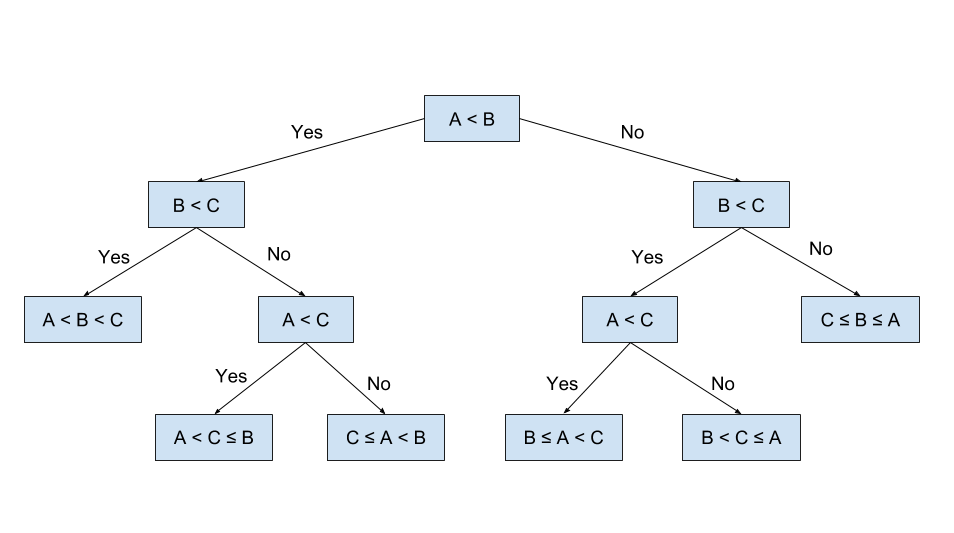
\includegraphics[width=120mm]{figures/decisionTree.png}
  \caption{Example of a basic decision tree}
  \label{decisionTree}
\end{figure}

A decision tree is where we sort the data by asking a sequence of questions and following the flowchart down to where it leads.
By the time we are at the bottom of the tree and have classified the data we can say exactly how the model does it's classification.
For instance if a decision tree is used for mortgage decisions and the model says no, we can query and learn that it said no because you had too low income or too low credit score for instance.

\begin{figure}[H]
  \centering
  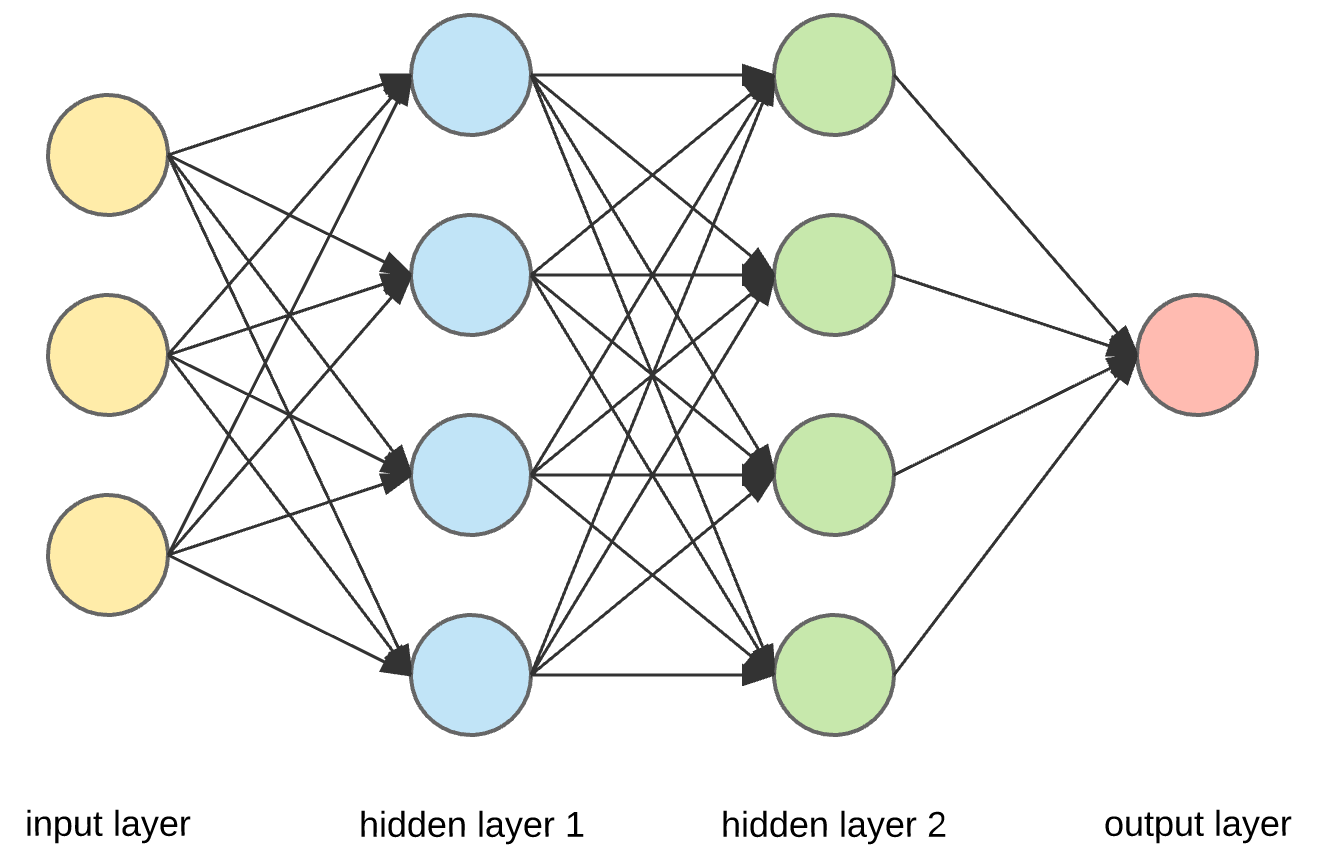
\includegraphics[width=120mm]{figures/neuralNet1.png}
  \caption{Example of a basic Neural Net}
  \label{neuralNet1}
\end{figure}

By contrast, a machine learning model like a neural net is almost a black box with regards to how the decisions are made.
We can query the model and ask it what it made its decisions based on, however, the features it picks out often isn't decipherable to humans in any way.
As in the previous example, if the answer to a mortgage is no, we have no real idea why the model made that decision.
That being said, neural networks are often able to come up with better outcomes for classification that simple models like decision trees are.
In the mortgage example, even if the neural net can't tell us how it comes to the conclusion of approving a loan, it is still more likely to be able to better tell who will be a good credit risk compared to the decision tree.
That's often the trade off that we make when deciding on a more opaque model.
That's why even though they are opaque in how they come up with their answers we still rely on them so heavily.
Because we can empirically test through monte-carlo studies how well they perform both in term of efficiency as well as how often these models misidentify the data that we are throwing at it.

While a neural network is opaque about how the decisions are made, the model itself doesn't have to be a black box for us.
We can take a peek under the hood and see how these models work.
To do so, we start up from the basic models like a perceptron and work our way to a graph neural network, finally connecting it to how neutrino reconstruction works.

\subsection{Perceptron Neuron}

A lot of things that seem incredibly easy to humans -- such as  recognizing the difference between say a cat and a dog -- are very difficult for computers to do.
What makes it difficult to make that sort of classification is that it is hard for humans to define concrete rules about what makes the picture of a cat different than the picture of a dog.
Neural nets approach this in a completely different fashion.

Instead of trying to define rules about the features that differentiate the picture of a dog vs a cat, we instead classify a whole bunch of pictures by hand.
\footnote{This is true only for supervised learning.
Unsupervised learning doesn't require classification by hand but have their own set of disadvantages}
Then throw those pictures at the algorithm with the correct answers and over time the computer learns to tell the difference between that of a dog and a cat.
We call an algorithm like this that separates things into two piles a binary classifier.
There are many different kinds of binary classifiers with a whole host of advantages and disadvantages but we will start with one that is simple to understand; the perceptron.

\begin{figure}[H]
  \centering
  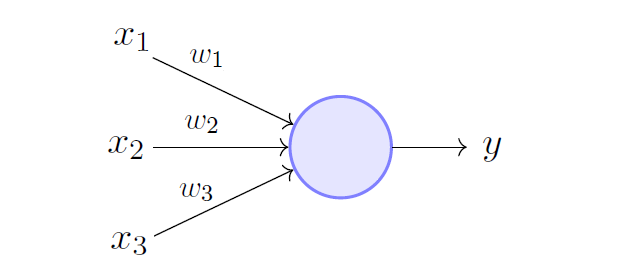
\includegraphics[width=120mm]{figures/perceptron1.png}
  \caption{Perceptron Neuron \cite{El-Amir_Hamdy_2019}}
  \label{perceptron1}
\end{figure}

A perceptron takes a number of inputs that are binary in nature and produce a single binary output \cite{Freund_Schapire_1998} ie.is this a dog? The figure \ref{perceptron1} has 3 inputs ($x_1$, $x_2$ and $x_3$) although, more or fewer inputs may be used.
Each input then is given a weight -- $w_1$, $w_2$ and $w_3$ in this case -- and the output calculated thus.

\begin{align}
  y = \begin{cases}
    0 \textrm{ if } \sum_i w_i x_i \leq \textrm{threshhold},\\
    1 \textrm{ if } \sum_i w_i x_i > \textrm{threshhold},\\
  \end{cases}
\end{align}

Used in this fashion, a perceptron can only make simple choices.
Raising the threshold makes the classification tighter while lowering it loosens the classification.
Because the output of a perceptron is binary, for more subtle distinctions, we can use the output of a perceptron to feed into the input of the next one thus creating a network that is more able to measure subtlety.

\begin{figure}[H]
  \centering
  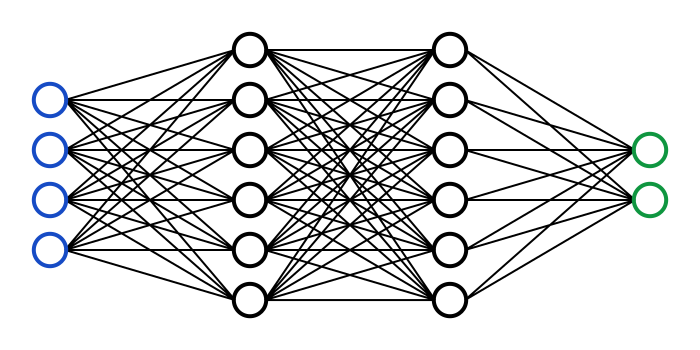
\includegraphics[width=120mm]{figures/network.png}
  \caption{Perceptron network \cite{Zhou_2020}}
  \label{network}
\end{figure}

Varying the weights of the inputs in combination with the threshold for the output allows us to get different models of classification.
The neurons in the first layer are only able to make simple decisions based on the raw input but because we use their output as the input to the second layer, the second layer can make more abstract decisions with a degree of subtlety impossible not only with one perceptron but also with even a single layer of perceptrons.
The complexity of the discrimination by the classifier increasing with both the number and layers of perceptrons in the network.

With the correct weights and threshold values, we can get any binary classifier we want using a set of perceptrons.
That, however, puts us back at our original problem of classifying whether something is a dog; namely, if we knew what features to look for (i.e.\ what weights and threshold to use) it wouldn't be hard explaining to a computer what a dog was.
The true innovation comes with using learning algorithms that don't require input from the programmer to set these weights and thresholds.

  If we want to use algorithms that can adjust weights and thresholds (otherwise called biases) automatically, we need some method where a small change in the weight only causes a small change in the output.
Because perceptrons are binary, this is impossible to do with only perceptrons.

  A small change in the weight to an input to the perceptron can flip the output entirely.
While this small change in weight can make one of the outputs of the network better, it may also affect the rest of the network behave in unpredictable ways.
Going back to the dog and cat example, while changing the weight slightly may make it better at recognizing dogs, it may wreak havoc on how cats are identified.

  This is where sigmoid neurons come in.

\subsection{Sigmoid Neuron}

While perceptrons are effectively step functions, flipping from $0$ to $1$, sigmoids are more smoothed out.
This means that a small change in the weight can lead to a small change in output\cite{Nielson_2020}.
The sigmoid function can be written as

\begin{align}
  \sigma = \frac{1}{1 + e^{-z}}
\end{align}

This means that a sigmoid neuron can be written as

\begin{align}
  \frac{1}{1 + e^{-\sum_i w_i x_i - b}}
\end{align}

where the $b$ stands for the bias of every input.
While this looks different than the perceptron at first glance it is just a more smoothed out version of it.
One key thing that we lose with the introduction of sigmoids is the linearity that perceptrons afforded us.
What we gain is the ability for our programs to automatically adjust their weights and biases because a small change in weights does lead to small change in output as shown in equation \ref{bias}.

\begin{align}\label{bias}
  \Delta y \approx \sum_i \frac{\partial y}{\partial w_i}\Delta w_i + \frac{\partial y}{\partial b}\Delta b
\end{align}

\begin{figure}[H]
  % https://blog.roboflow.com/activation-function-computer-vision/
  \centering
  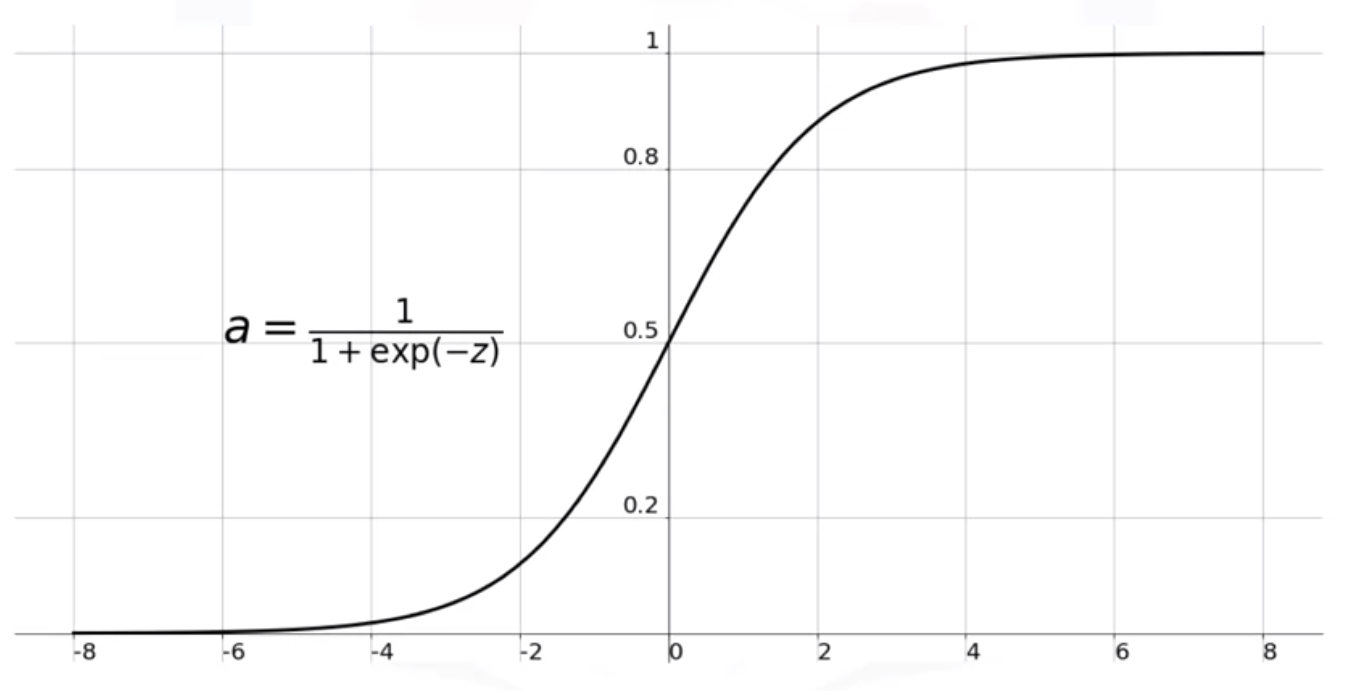
\includegraphics[width=80mm]{figures/sigmoid.png}
  \caption{Sigmoid Function \cite{Potrimba_2023}}
  \label{network}
\end{figure}

More than the exact formula of the sigmoid neuron what matters is the shape.
As a result, other neurons can be used in its stead which retain the property of having a small change in weight lead to a small change in output.
Some of the more popular of these functions (called activation functions) are RELU and softmax.
Each have their own advantages and disadvantages and may even be mixed in the same neural network


 